\documentclass[a4paper,10pt,oneside]{article}
$
\usepackage[polutonikogreek,italian]{babel}
$
\usepackage[utf8x]{inputenc}
$
\usepackage{amsmath}
$
\usepackage{amsthm}
$
\usepackage{amssymb}
$
\usepackage{amscd}
$
\usepackage[pdftex,colorlinks=true,urlcolor=black]{hyperref}
$
\usepackage{graphicx}
$
\usepackage{float}
$
\usepackage{array}
$
\usepackage{rotating}
$
\usepackage[small]{caption}
$
\usepackage{lscape}
$
\usepackage{fancybox}
$
\usepackage{booktabs}
$
\usepackage[noanswer]{exercise}
$
\parindent0ex
$
\renewcommand{\fboxsep}{0.4cm}
$
\renewcommand{\textfraction}{0.05}
$
\renewcommand{\topfraction}{0.95}
$
\renewcommand{\bottomfraction}{0.95}
$
\renewcommand{\floatpagefraction}{0.35}
$
\renewcommand{\ExerciseName}{Esercizio}
$
\renewcommand{\ExerciseListName}{Es}
$
\setcounter{totalnumber}{5}
$
\restylefloat{figure}
$
\begin{document}
$
\section*{Esempi ed elementi di teoria della misura}
$
\begin{figure}[H]
 \centering
 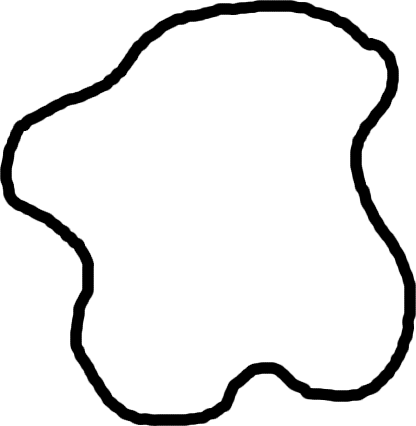
\includegraphics[width=.7\textwidth]{../immagini/superficieIrregolare.png}
 % superficieIrregolare.png
 \label{fig:superficieIrregolare}
\end{figure}


$
\subsection*{Il processo di misura}
$
\subsubsection*{Una misura diretta di superficie}
$

$
L'immagine nel riquadro rappresenta il profilo di una superficie piana di forma irregolare.
$
Utilizzando un foglio di carta semitrasparente, acquisite un calco fedele del profilo ed appoggiatelo su un foglio
$
quadrettato in modo ragionevolmente sottile (per esempio, con un passo di 4 o 5 millimetri).
$
Ciascuno studente, conteggi diligentemente il numero dei quadretti completamente interni al proprio calco, scartando
$
quelli esterni e quelli che toccano anche in un solo punto il bordo.
$
\newline
$

$
Se avete operato in modo sufficiente attento e sufficientemente {\bfseries {\slshape indipendente}}, il numero dei
$
quadretti conteggiati sarà diverso per ciascun osservatore.
$
\newline
$

$
Discutete, ragionando tra di voi e con il vostro insegnante, sulle cause di questo fenomeno.
$
Contemporaneamente, usate questo esempio per riflettere sui problemi e le caratteristiche di un processo di misura.
$
\newline
$

$
Essenzialmente, la misura è una delle forme con le quali l'uomo, in fisica, osserva i fenomeni naturali. In modo
$
generico, si potrebbe sostenere che ogni affermazione fisica è il risultato di una misura nascosta. Per esempio, la
$
frase
$
{\slshape Tutti gli oggetti pesanti cadono verso il suolo}, nasconde la misura della direzione del moto di caduta e una
$
stima del peso necessario ai corpi per sottostare al comportamento descritto, distinguendoli
$
{\slshape quantitativamente} dai corpi leggeri. Tecnicamente, invece, la parola misura si riferisce all'operazione
$
con la quale viene associato un numero ad un determinato aspetto
$
misurabile di un fenomeno fisico (la {\slshape grandezza}). Questa operazione, tuttavia, non è sempre
$
immediata, come saremmo portati a pensare,  ma può riservare problemi e sorprese, come nell'esempio della nostra
$
superficie.
$
\newline
$

$
Se vogliamo cercare una definizione sintetica, potremmo dire che:
$

$
\begin{quote}
$
\bfseries{
$
una misura è il processo sperimentale con il quale un fisico determina alcune proprietà del sistema osservato, esprimendole in
$
termini matematici.
$
}
$
\end{quote}
$

$

$

$

$
\subsubsection*{Attività}
$

$
Immaginiamo di dover {\bfseries misurare un banco} .
$

$
Come possiamo procedere?
$

$
Ciascuno studente, in modo {\bfseries{\slshape indipendente}}, cioè senza consultare i compagni, annoti sul quaderno i
$
seguenti elementi:
$
\begin{itemize}
$
\item Gli strumenti necessari per misurare il banco;
$
\item Le operazioni principali del processo di misura;
$
\item Una stima del risultato atteso.
$
\end{itemize}
$
Al termine, confrontare le proposte con il contributo dell'insegnante.
$

$
\subsubsection*{Le grandezze fisiche}
$
Ogni fenomeno fisico coinvolge un insieme numeroso di proprietà distinte.
$
\newline
$

$
Un cavallo al galoppo occupa in ogni istante un punto diverso della pista. Per descriverne il moto è necessario
$
effettuare delle misure di {\bfseries tempo} e di {\bfseries spazio}.
$

$
Lungo la corsa, il cavallo solleva schizzi di fango dalle pozzanghere sul terreno. Da essi possiamo ricavare
$
informazioni sugli scambi di {\bfseries quantità di moto}, e distinguere, tra più animali, il {\bfseries più pesante} o
$
il {\bfseries più veloce}.
$

$
Ancora, il cavallo suda. Perciò aumenta la propria {\bfseries temperatura} corporea e scambia {\bfseries calore} con
$
l'ambiente.
$
\newline
$

$
Un tempo si può misurare in secondi, mesi o in anni. Una lunghezza può essere misurata in metri, chilometri, miglia o
$
in anni luce. Ogni misura descrive una grandezza riferendosi a un ben preciso elemento di paragone, chiamato unità di misura.
$
L'indicazione dell'unità di misura è un elemento indispensabile per dare senso compiuto a qualunque misura fisica.
$

$
Continuate la descrizione individuando nuove proprietà misurabili e ripetete il gioco per nuovi fenomeni indipendenti,
$
avendo cura di identificare sistematicamente la {\slshape proprietà misurabile} e il nome della {\slshape grandezza
$
fisica} corrispondente.
$

$
Al termine, confrontate le proposte dei singoli, per discuterle con l'insegnante.
$

$
\subsection*{L'elaborazione dei dati}
$
Un fruttivendolo appoggia le mele sul piatto della bilancia e legge sul display peso e costo della merce.
$
\newline
$

$
La fisica non può accontentarsi di una rilevazione sommaria ed affrettata delle misure, ma le valuta criticamente in un
$
modo più attento. Nell'esempio della superficie irregolare, mostra una situazione
$
concreta nella quale un processo di misura produce, per un singolo oggetto, più risultati differenti. È compito
$
del fisico, in queste
$
situazioni, dare un senso all'informazione raccolta, superando l'apparente confusione iniziale.
$
Il processo che porta a questa
$
sintesi si chiama {\bfseries analisi dei dati}.
$
\newline
$

$
A volte, una buona analisi dei dati richiede procedure molto complesse. Nel nostro esempio, invece, possiamo individuare
$
un insieme di operazioni semplici e sensate che ci permettono di procedere. 
$
\begin{enumerate}
$
\item Ordinate tutti i risultati raccolti su una colonna, dal maggiore al minore, contrassegnando le eventuali misure
$
ripetute.
$
\item Calcolate la differenza tra il valore massimo e il valore minimo della misura. Il risultato può essere chiamato
$
{\bfseries dispersione (assoluta) della misura}.
$
\item Valutate se, a vostro giudizio, questo valore può essere ritenuto grande o piccolo. Un modo comune di fare questo
$
è dividere la dispersione assoluta della misura per uno dei risultati della misura stessa. In questo caso si parla di
$
{\bfseries dispersione relativa}.
$
\item Rappresentate i dati in una {\bfseries curva di frequenza}, realizzata come segue:.
$

$
Rappresentate in ascissa l'intervallo di dispersione dal valore minimo misurato a quello massimo e suddividetelo in un
$
piccolo numero di parti. Se avete venti misure, ad esempio, può bastare una suddivisione in quattro o cinque settori.
$

$
Per ogni settore riportate, in ordinata, il numero di ricorrenze della misura nell'intervallo corrispondente.
$

$
Discutete il grafico con l'insegnante, in particolare cercate di valutare se è possibile riconoscere qualche tipo di regolarità.
$
\item Riflettete sul grado di omogeneità dei vostri dati. Sicuramente, li avrete acquisiti usando sempre la stessa diligenza e la stessa
$
attenzione, tuttavia, in questo caso, non è possibile attribuire a tutti i dati lo stato grado di affidabilità. Scegliete ad esempio
$
due misure per difetto. Trattandosi necessariamente di valori più piccoli del valore vero della vostra superficie, potete riconoscere
$
con certezza quale delle due è più vicina alla misura cercata. Questo non significa necesariamente che l'operatore che ha ricavato il
$
dato sia stato più bravo, ma semplicemente più fortunato.
$

$
Da ciò, tuttavia, discende una conseguenza importante. Se i dati disponibili non hanno lo stesso grado di omogeneità, non sarà oportuno operare
$
su di essi una media matematica. Anzi, eseguendo la media dei dati, si otterrebbero valori peggiori di quelli già disponibili.
$
\item Se non è possibile effettuare una media matematica, significa che è stato inutile ripetere più volte la misura, o ritenete che la ripetizione abbia
$
comunque consentito di migliorare la misura finale? Esprimete la vostra opinione.
$
\item Discutendo tra voi e con l'insegnante, definite il modo più opportuno per eprimere il risultato finale del vostro lavoro.
$

$
\end{enumerate}
$

$
\subsection*{Rappresentare i numeri in fisica}
$
In fisica, i numeri hanno un significato molto diverso che in matematica.
$
\newline
$

$
Un autista sufficientemente attento può mantenere con facilità il veicolo ad una
$
velocità costante prefissata, ad esempio di 50 km/h, per un lungo intervallo di
$
tempo. Tuttavia, non è assolutamente detto che un sensore di velocità
$
indipendente, collocato sui bordi della strada, debba rilevare necessariamente
$
lo stesso identico valore di 50 km/h, al passaggio dell'autoveicolo.
$

$
Il motivo risiede nel fatto che il tachimetro dell'automobile, così come i
$
sensori di velocità commerciali d'uso comune, hanno una precisione che si
$
aggira intorno al 5\%, ma riportano il dato con una sensibilità superiore alle
$
proprie caratteristiche.
$
\newline
$

$
Quindi, pur leggendo il 50 sul proprio tachimetro, l'autista potrebbe
$
indifferentemente affermare di viaggiare a 48 km/h, piuttosto che a 52 km/h,
$
senza commettere una falsificazione oggettiva del dato.
$
\newline
$

$
In altre parole, il risultato di una misura è un numero privo di significato se
$
non accompagnato da una stima dell'{\bf errore}, perché una misura
$
identifica {\slshape sempre} un {\bf intervallo di valori} (e non un singolo valore numerico).
$
Per indicare correttamente questa proprietà, il risultato della misura dovrebbe essere
$
rappresentato da una forchetta, in uno di questi modi:
$

$
\begin{center}
$
\begin{math}
$
47,5 \frac{km}{h} < v < 52,5 \frac{km}{h}
$
\end{math}
$
oppure
$
\begin{math}
$
v = 50 \frac{km}{h} \pm 2,5 \frac{km}{h}
$
\end{math}
$
\end{center}
$
$
\subsubsection*{Le cifre significative e la notazione scientifica}
$
Un cubetto di rame di un centimetro cubo contiene, allineati in modo regolare su ciascuno spigolo, cento milioni di
$
atomi. In tutto, sono 1000000000000000000000000 atomi. Ciascuno di essi occupa un volume di 
$
0,000000000000000000000000000001 \begin{math}m^3\end{math}.
$

$
La fisica si interessa di fenomeni molto piccoli e di fenomeni molto grandi, e ha la necessità di scriverli in un modo
$
espressivamente efficace. Come nei due esempi qui sopra, la notazione decimale è particolarmente scomoda, appena si
$
evade dall'uso quotidiano dei prezzi al supermercato o dei problemi didattici dei nostri libri di testo. Già i
$
matematici, quando incontrano un numero importante, sono abituati a sostituirlo con un simbolo, perché la notazione
$
decimale è troppo pesante e di scarso interesse.
$

$
In fisica, un numero deve contemporaneamente, essere facile da leggere, da capire e da usare per scopi {\slshape
$
operativi}. Per questo, è necessario distinguere, nella scrittura, le parti importanti da quelle trascurabili,
$
attraverso un insieme di convenzioni e regole specifiche.
$
\newline
$

$
Un primo problema, è quello di trovare una convenzione capace di incorporare l'errore nella scrittura del risultato.
$

$
In precedenza, infatti, abbiamo descritto il metodo della forchetta, che è sicuramente il modo più efficace e corretto
$
di separare la stima del valor vero di una misura dall'errore associato. In certe situazioni, quando non serve essere
$
troppo rigorosi, si preferisce usare la convenzione delle cifre significative. Nell'esposizione di un
$
risultato\footnote{in notazione decimale} si scrivono solo quelle parti del numero che si ritiene di avere misurato con
$
sicurezza.
$
\newline
$

$
Supponiamo di effettuare una misura di lunghezza con un righello da cartoleria.
$
In questo caso la precisione della misura è pari al passo del righello, cioè un
$
millimetro. Allora indicheremo il risultato in questo modo:
$
\begin{center}
$
	\begin{math}
$
      		L_{righello}\;=~12,5~cm
$
	\end{math}
$
		oppure
$
	\begin{math}
$
		L_{righello}~125~mm
$
	\end{math}
$
\end{center}
$
Se, successivamente, dovessimo rivalutare la stessa misura con l'uso di un
$
calibro, e se ottenessimo esattamente lo stesso risultato, lo dovremmo scrivere
$
in un modo diverso, evidenziando la maggior precisione:
$

$
\begin{center}
$
	\begin{math}
$
		L_{calibro}~=~12,50~cm
$
	\end{math}
$
		oppure
$
	\begin{math}
$
		L_{calibro}~= ~ 125,0~ mm
$
	\end{math}
$
\end{center}
$

$
Un riferimento di buona qualità, per approfondire il concetto di cifre significative e per fare
$
qualche esercizio, si può trovare all'interno del sito web dell'Università di Messina\footnote{
$
\url{http://ww2.unime.it/cclchim/generale/significative.htm}}
$
\newline
$

$
Un secondo problema, legato alla scrittura di un numero, è quello di trasmettere a prima vista la percezione della
$
dimensione, affinché sia possibile confrontarlo rapidamente con altri numeri più grandi o più piccoli. Il volume di un
$
atomo, ad esempio, non deve {\bf mai} essere scritto come abbiamo fatto sopra, altrimenti risulta impossibile sia da
$
leggere che da usare.
$
Una tecnica molto utile è la {\bf notazione scientifica}. Ogni numero viene separato in due parti. La più importante è
$
senz'altro l'ordine di grandezza. Lo spazio occupato da un atomo in un reticolo cristallino, ad esempio, diventa
$
semplicemente \begin{math}10^{-30}~m^3\end{math} e la densità degli atomi sarà di \begin{math}10^{24}
$
atomi/cm^3\end{math}.
$

$
In questi esempi, gli zeri non sono cifre significative. Invece di scriverli tutti, è molto meglio contarli!
$
\newline
$

$
Consideriamo ora un esempio di come l'uso della notazione scientifica permette di superare alcune ambiguità che la
$
notazione decimale lascerebbe irrisolte, nell'indicazione delle cifre significative.
$
\newline
$

$
Immaginiamo di misurare
$
a passi la lunghezza di un campo di calcio. Supponiamo di avere misurato 100
$
passi e che un singolo passo possa essere stimato uguale a 1,1 metri, con una
$
precisione intorno al 10\%. Esprimendo il risultato con una forchetta potremmo
$
scrivere:
$

$
\begin{center}
$
	\begin{math}
$
		100~m~ <~ L~ <~ 120~ m
$
	\end{math}
$
\end{center}
$
Per come è stato posto il problema, noi siamo in grado di riconoscere, nella lunghezza del campo, i decametri, ma non i
$
metri. Se esprimiamo il risultato in metri, con la notazione decimale, le prime due cifre sono significative e la terza
$
no.
$

$
Se usiamo la notazione decimale, scrivendo \(L~= ~ 110~ m\), siamo costretti ad utilizzare una cifra
$
significativa in più del necessario e quindi dichiariamo un risultato {\slshape gravemente} (sic!)
$
errato.
$
\newline
$

$
 Per evitare questo problema, esistono essenzialmente due modi:
$

$
\begin{itemize}
$
\item Rinunciare all'uso del metro come unità di misura, sostituendo con un
$
multiplo adeguato. Per esempio:
$

$
\begin{center}
$
	\begin{math}
$
		L~ = ~ 0,11~ km
$
	\end{math}
$
\end{center}
$
\item Usare la notazione scientifica, scrivendo:
$
\begin{center}
$
	\begin{math}
$
		L~ = ~11~ *~ 10^1~ m
$
	\end{math}
$
\end{center}
$
\end{itemize}
$

$
Per approfondire il concetto di
$
notazione scientifica potete trovare moltissimi riferimenti. Proviamo qui a indicare la definizione di {\itshape
$
\href{http://www.wikipedia.org/wiki/Notazione_scientifica}{wikipedia}} e
$
discutetela con l'insegnante\footnote{n.d.a: per la verità, a tutto il 3 luglio 2011, quella definizione
$
\`e piuttosto carente. Ne proponiamo la lettura perché, a nostro parere dovrebbe essere rivista da qualche studente di
$
buona
$
volontà.}.
$

$
\subsubsection*{Campioni e unità di misura}
$

$
Una misura è un'operazione di confronto.
$

$
Per esempio, la misura di superficie all'inizio di questo capitolo era
$
il confronto tra la dimensione di un quadretto di quaderno. Nel nostro esercizio, il quadretto era un campione che
$
svolgeva la funzione di unità di misura.
$
\newline
$

$
Concettualmente, la scelta dell'unità di misura è attribuita alla libera scelta dell'operatore che esegue la misura ma,
$
agli effetti pratici, è necessario fare riferimento a delle convenzioni riconosciute. La scelta dell'unità di misura,
$
in questo caso, è deferita alle disposizioni di un'autorità riconosciuta.
$
\newline
$

$
Quando una grandezza viene confrontata con il campione, si esegue una misura diretta.
$
Sempre in riferimento all'attività del primo paragrafo,
$
proviamo a descrivere una ad una le singole operazioni necessarie
$
per realizzare una misura diretta, come se dovessimo generare un algoritmo per
$
programmare un computer. Forse potremmo operare così:
$
\begin{enumerate}
$
\item Produciamo una superficie di prova\( ~\mathcal{P}\);
$
\item Confrontiamo la superficie $~\mathcal{S}$ ad con un singolo quadretto;
$
\item Se la superficie è maggiore del quadretto aggiungiamo un quadretto a
$
$~\mathcal{P}~$ e riportiamoci al punto 2);
$
\item altrimenti poniamo \(~\mathcal{S}~ = ~\mathcal{P}~ \) ed usciamo.
$
\end{enumerate}
$

$
In generale, quando si esprime il risultato di una misura, si assume sempre di
$
avere eseguito una vera e propria misura diretta.
$
\newline
$

$
Ma, nella pratica, non sempre è cos\'i.
$
\newline
$
Per esempio, la distanza tra la terra e il Sole è pari a $~150~10^{12}~m~$
$
(centocinquantamila miliardi di metri !). Il metro campione è conservato
$
all'Ufficio internazionale pesi e misure di Sevres, vicino a Parigi, ed è lungo
$
circa un paio di gomiti. Non vorrete pensare di mandarci il vostro compagno di banco,
$
a misurare in modo diretto la distanza terra-Sole, con il metro campione di
$
Parigi ...
$
\newline
$

$
Il campione di misura è detto anche {\bf unità di misura}. Per
$
convenzione, la comunità scientifica ha selezionato alcune unità di
$
misura convenzionali\footnote{secondo un meccanismo determinato dal cosiddetto
$
Sistema Internazionale di unità di misura, che è descritto al paragrafo successivo}
$
per tutte le grandezze d'uso più
$
comune. Tuttavia è spesso opportuno, per facilitare la comprensione dei fenomeni
$
studiati, utilizzare dei multipli o dei sottomultipli dell'unità di misura di
$
riferimento.
$
\newline
$
Per esempio, per le lunghezze, l'unità di misura convenzionale è il metro, ma
$
spesso le misure di lunghezza sono espresse in chilometri, in ettometri, in
$
decametri, in centimetri, in millimetri, in micron e così via. Un chilometro
$
equivale a mille metri, e viene rappresentato con l'uso del prefisso {\bf k}:
$

$
\begin{center}
$
\begin{math}
$
1~km~=~10^3~m
$
\end{math}
$
\end{center}
$
Il millimetro corrisponde a un millesimo di metro (sottomultiplo), e viene
$
rappresentato con l'uso del prefisso {\bf m}:
$

$
\begin{center}
$
\begin{math}
$
1~km~=~10^{-3}~m
$
\end{math}
$
\end{center}
$
Ancora, il ${\bf Gm}$ (gigametro) corrisponde a un miliardo di metri, il ${\bf Mm}$
$
(megametro) a un milione di metri, il ${\mathbf \mu m}$ (micrometro) a un milionesimo di
$
metro (cioè un millesimo di millimetro) e il ${\bf nm}$ (nanometro) a un miliardesimo
$
di metro. Per una lista più ampia, consultate wikipedia
$
\footnote{
$
\url{http://it.wikipedia.org/wiki/Sistema_internazionale_di_unit\%C3\%A0_di_misura\#Prefissi}}
$
.
$

$
\subsubsection*{Il sistema Internazionale delle Unità di Misura}
$
Lo spettro di fenomeni a cui la fisica si interessa è vastissimo, ed è altrettanto vasto
$
l'insieme delle grandezze osservabili necessarie per rappresentarlo.
$

$
La Comunità Scientifica ha ritenuto necessario stabilire un po' d'ordine sulla questione, incaricando
$
un organismo riconosciuto a livello internazionale di definire i nomi convenzionali delle grandezze,
$
i simboli relativi e le unità di grandezza standard a cui fare riferimento.
$
\newline
$

$
Questo orgnaismo si chiama Ufficio Internazionale dei Pesi e delle Misure (acronimo: {\bf BIPM}, è un'organizzazione senza
$
scopo di lucro, con sede in Francia, che ha questo sito di riferimento:
$
\newline
$

$
\url{http://www.bipm.org}
$
\newline
$

$
Come puoi verificare anche usando wikipedia\footnote{
$
\url{http://it.wikipedia.org/wiki/Sistema_internazionale_di_unit\%C3\%A0_di_misura}
$
\newline
$

$
}
$
il sistema internazionale (acronimo: {\bf SI}) individua un insieme limitato di unità di misura
$
fondamentali, che sono la {\bf lunghezza}, il {\bf tempo}, la {\bf massa} e l'{\bf intensità di corrente}.
$
\newline
$
Queste unità sono, rispettivamente il {\bf metro}, il {\bf secondo}, il {\bf chilogrammo massa} e
$
l'{\bf Ampere}.
$
\newline
$
\newpage
$
Per ciascuna di esse il {\bf BIPM} definisce un'unità di misura fondamentale, di cui stabilisce la definizione rigorosa.
$
\newline
$

$
Si tratta di una definizione soggetta a modificazioni nel tempo, inseguendo l'evoluzione del progresso tecnologico.
$
\newline
$
Attualmente\footnote{
$
\url{http://www.bipm.org/en/si/base_units/metre.html}
$
}:
$
\begin{center} \bf The metre is the length of the path travelled by light in vacuum during a time interval of 1/299
$
792 458 of a second.
$
\end{center}
$

$
La definizione originale dell'unità di misura del metro lineare, invece, possiede una storia affascinante\footnote{
$
\url{http://www.bipm.org/en/si/history-si/evolution_metre.html}
$
}.
$
\newline
$
Fu determinata, infatti, nel 1799, in piena rivoluzione francese, in funzione delle dimensioni della circonferenza
$
terrestre. Si stabilì, infatti, che un quarto dell'asse terrestre dovesse corrispondere a $10^7 m$ (dieci milioni di
$
metri). Siccome, in radianti, un quarto di circonferenza corrisponde a {\boldmath $\frac{\pi}{4}$}, rimane definita
$
automaticamente la misura del raggio terrestre, secondo la formula $\frac{C}{4}~=~\frac{\pi}{4}r~=6.3~10^3 km$.
$

$
L'iniziativa transalpina nella definizione delle unità di misura fondamentali fu oggetto di contestazioni per eccesso
$
di protagonismo da parte della comunità scientifica di area anglosassone, e non fu accettata completamente. Ancora
$
oggi, sebbene le convenzioni internazionali siano solidamente riconosciute ovunque, molte unità di misura del sistema
$
SI sono sostituite di fatto, nell'uso comune di molti stati nazionali che gravitano l'area del
$
Commonwealth Britannico, inclusi gli Stati Uniti, da unità di misura alternative\footnote{ecco uno dei tanti siti che
$
riportano una tabella di conversione tra unità standard e unità convenzionali:\newline
$
\url{http://www.oppo.it/tabelle/unita_misura_conversioni.htm}}
$
, come il pollice, il piede, la
$
iarda, il miglio (marino e terrestre), il gallone, la libbra, l'oncia ...
$
\newline
$

$
In fisica, l'uso delle unità di misura non standard non dovrebbe essere assolutamente {\itshape mai} usato, se non per
$
qualche salutare esercizio di conversione tra unità di misura.
$
$
\subsubsection*{Misura non ripetibile di lunghezza}
$

$
  \begin{figure}[H]
$
  \centering
$
   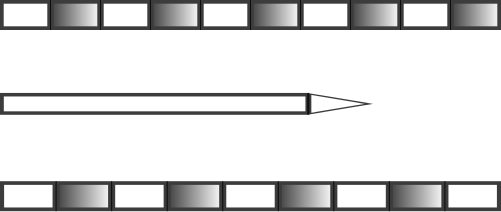
\includegraphics[width=\textwidth]{../immagini/mozzicone.png}
$
   \label{figure:nonio}
$
   \caption{il nonio decimale}
$
  \end{figure}
$

$
In figura \ref{figure:nonio} osserviamo un mozzicone di matita tra due regoli graduati, che
$
vogliamo utilizzare come strumenti per una misura didattica della lunghezza del mozzicone.
$
\newline
$

$
Prima di tutto, osserviamo i due strumenti di misura. Si tratta di due righelli graduati con un passo
$
diverso. Infatti, pur avendo la stessa lunghezza totale, contano uno nove unità e il secondo dieci. Il primo righello,
$
di conseguenza, possiede una {\bf sensibilità} {\bf u} leggermente inferiore alla sensibilità {\bf v} del secondo.
$

$
Possiamo determinare una prima misura della lunghezza della matita in uno di questi due modi:
$

$
\begin{center}
$
  \begin{math}
$
    8~v~<~L~<~9~u~~~~oppure~~~~L~=~8.5~\pm ~0,5~u
$
  \end{math}
$
\end{center}
$
\begin{center}
$
  \begin{math}
$
    7~u~<~L~<~8~v~~~~oppure~~~~L~=~7.5~\pm ~0,5~v
$
  \end{math}
$
\end{center}
$

$
La prima misura è affetta da un errore relativo $\Delta L~=~\frac{v}{L}~=~frac{1}/{8}=0.13~=~13\%$, e la seconda da un
$
errore relativo $\Delta L~=~\frac{v}{L}~=~frac{1}/{7}=0.14~=~14\%$. Oggettivamente non è granché, ma non possiamo far
$
meglio per questi motivi:
$
\begin {itemize}
$
\item I regoli sono graduati con un passo grossolano e quindi sono poco sensibili.
$
\newline
$
Probabilmente, il vostro occhio (che
$
è più sensibile delle barre graduate) è in grado di proporre una stima migliore, ma per riuscirci siete costretti a
$
cercare dei riferimenti (cioè degli strumenti di misura) aggiuntivi. Noi dobbiamo riflettere
$
esclusivamente sulle proprietà dei righelli.
$
\item Il nostro metodo di misura è piuttosto ingenuo e non sfrutta adeguatamente gli strumenti disponibili.
$
\newline
$
Infatti, entrambi i regoli sono allineati alle estremità di sinistra con
$
la matita, come siamo sempre stati abituati a fare. Questa scelta è molto comoda, perché ci dà
$
certezza che,
$
ripetendo cento volte la misura allo stesso modo, otterremmo cento volte lo stesso risultato. In termini tecnici, si
$
dice che abbiamo scelto di effettuare una misura {\bf non ripetibile}.
$
\end{itemize}
$

$
Vediamo ora come, modificando di poco il {\slshape metodo} di misura, è possibile migliorarne la qualità.
$
\newline
$
Dopo aver riprodotto fedelmente una delle due scale su una striscia di carta, allineate un'estremità della striscia
$
alla punta della matita, come nella figura \ref{figure:nonio2}.
$
Adesso le tacche iniziali della due strisce sono disallineate tra loro, di una quantità uguale allo spazio
$
contrassegnato in figura con {\bf x}. {\bf x} è l'errore della nostra misura. Ma siccome rappresenta una
$
quantità inferiore al passo del regolo, fino ad ora non abbiamo potuto valutarla.
$
\newline
$
Se considerate ora, a due a due, le
$
tacche successive, vi accorgerete che il disallineamento si riduce di molto. Questo accade perché le unità delle due
$
scale sono differenti di un decimo tra loro. In particolare, la scala che abbiamo spostato a fianco della matita
$
utilizza unità più lunghe, quindi tende ad avvicinare le proprie tacche alla striscia precedente di un piccolo passo.
$
Quando osserviamo la sovrapposizione la striscia superiore è rimasta indietro per 6 volte successive, cioè 6 decimi
$
della propria lunghezza. Aggiungendo questi 6 decimi alla distanza distanza incognita si ottiene esattamente una unità.
$
Potremmo rappresentare questa affermazione con l'equazione seguente:
$
\begin{center}
$
\begin{math}
$
x~+6~\frac{u}{10}~=~u
$
\end{math}
$
\end {center}
$
 Quindi, possiamo concludere che il mozzicone oltrepassa di 4 decimi di unità e scriveremo:
$
\begin{center}
$
  \begin{math}
$
    7.35~u~<~L~<~7.45~u~~~~oppure~~~~L~=~7.4~\pm ~0,05~u
$
  \end{math}
$
\end{center}
$

$
  \begin{figure}[H]
$
  \centering
$
   \includegraphics[width=\textwidth]{../immagini/mozzicone2.png}
$
   \label{figure:nonio2}
$
   \caption{il nonio decimale}
$
  \end{figure}
$
Se avete capito:
$
\begin{itemize}
$
\item Calcolate la precisione di questa nuova misura.
$
\item Ripetete la misura spostando la striscia superiore, anzichè
$
quella inferiore e cercate di capire come bisogna adattare il procedimento\footnote{scoprirete che è più comodo.}.
$
\item Esprimete i risultati nelle unità di
$
misura {\bf v} della striscia composta di nove elementi.
$
\end{itemize}
$

$

$
La tecnica illustrata è alla base del funzionamento del nonio\footnote{
$
\url{http://it.wikipedia.org/wiki/Nonio_(strumento_di_misura)}} e del
$
calibro\footnote{\url{http://it.wikipedia.org/wiki/Calibro}}, strumenti che permettono di misurare lunghezze con una
$
risoluzione superiore alle possibilità dell'occhio umano.
$

$
\subsubsection*{Le Misure indirette}
$
Preparate un recipiente di forma regolare (per esempio un parallelepipedo a base rettangolare) e riempitelo d'acqua
$
fino a circa metà. Prendete un sasso irregolare di dimensioni opportune e immergetelo nell'acqua. Osservando
$
l'innalzamento del livello, cercheremo di ricavare il volume del sasso e la precisione della misura.
$
\newline
$

$
In questo caso la situazione non si presta, come in precedenza, a una misura diretta, perché non possediamo nessun
$
campione di volume da utilizzare come unità di misura. Però, siccome la forma del recipiente è regolare, possiamo
$
ricavare il volume da un insieme di misure di lunghezza. Quando una grandezza viene ricavata da misure di grandezze
$
diverse, non omogenee, attraverso una serie di calcoli matematici, si dice di aver eseguito una misura indiretta.
$

$
Prima di tutto, ricaviamo la superficie del rettangolo d'acqua dalla misura dei suoi lati, diciamo ${\mathbf
$
{\overline{l_1}}}$ e ${\mathbf {\overline{l_2}}}$. Accontentiamoci di eseguire una sola misura non ripetibile, ma
$
teniamo conto con attenzione del corrispondente errore di misura, scrivendo quindi:
$
\begin{center}
$
\begin{eqnarray}
$
l_1~=~\overline{l_1}~\pm~\Delta l_1 \\
$
l_2~=~\overline{l_2}~\pm~\Delta l_2 \nonumber
$
\end{eqnarray}
$
\end{center}
$

$
Prima di determinare il valore di $\overline S$, osserviamo la seguente figura:
$

$
  \begin{figure}[H]
$
  \centering
$
   \includegraphics[width=\textwidth]{../immagini/propagazioneDegliErrori.png}
$
   \label{figure:propagazioneDegliErrori}
$
   \caption{La propagazione delgli errori}
$
  \end{figure}
$

$
Nella figura, la superficie misurata è quella tratteggiata. gli errori di misura possono spostare il vertice in alto a
$
sinistra in un punto qualunque del rettangolino verde. Quindi, il più piccolo valore possibile per la misura è:
$
\begin{center}
$
\begin{math}
$
S_{min}~=~(\overline{l_1}~-~\Delta l_1)(\overline{l_2}~-~\Delta l_2)
$
\end{math}
$
\end{center}
$
e il maggiore:
$
\begin{center}
$
\begin{math}
$
S_{max}~=~(\overline{l_1}~+~\Delta l_1)(\overline{l_2}~+~\Delta l_2)
$
\end{math}
$
\end{center}
$

$
Il valore centrale, invece, è semplicemente:
$
\begin{center}
$
\begin{math}
$
\overline{S}~=~\frac{S_{min}+S_{max}}{2}~=~\overline{l_1}~\overline{l_2}
$
\end{math}
$
\end{center}
$

$
Prima di definire l'errore, osserviamo meglio la figura. A rigore, l'errore corrisponde alla fascia esterna, composta
$
da tre rettangoli. Quello centrale, però è molto più piccolo degli altri. Infatti si ottiene moltiplicando tra loro i
$
due errori assoluti. In matematica, la moltiplicazione di due quantità piccole è una quantità estremamente piccoli.
$
Spesso, il rettangolo rosso è così piccolo che è possibile trascurabile del tutto, nella stima dell'errore su $S$.
$
Perciò scriveremo:
$
\begin{center}
$
\begin{math}
$
\Delta S~=~\overline{l_1}~\Delta l_2~+\overline{l_2}~\Delta l_1
$
\end{math}
$
\begin{equation}
$
S~=~\overline{S}~\pm~\Delta S~=~\overline{l_1}~\overline{l_2}~\pm~(\overline{l_1}~\Delta l_2~+~\overline{l_2}~\Delta l_1)
$
\end{equation}
$
\end{center}
$
A questo punto, possiamo passare allo studio del volume. Anche in questo caso, ci troviamo davanti ad una
$
moltiplicazione.
$
\begin{center}
$
\begin{math}
$
V~=S~h
$
\end{math}
$
\end{center}
$
Se la struttura matematica è la stessa, procederemo allo stesso modo di prima:
$
\begin{center}
$
\begin{eqnarray}
$
\overline{V}~=~\overline{h}~\overline{S} \nonumber \\
$
\Delta V~=~\overline{h}~\Delta S~+~\overline{S}~\Delta h
$
\end{eqnarray}
$
\end{center}
$
Prima di concludere, effettuamo il calcolo degli errori relativi.
$
\newline
$
Per la superficie:
$
\begin{center}
$
\begin{equation}
$
\epsilon_S~=~\frac{S}{\overline{S}}
$
=\frac{\overline{l_1}~\Delta l_2~+~\overline{l_2}~\Delta l_1}{\overline{l_1}*~\overline{l_2}}
$
~=~\frac{\Delta l_2}{\overline {l_2}}~+~\frac{\Delta l_1}{\overline{l_1}}
$
\end{equation}
$
\end{center}
$
Per il volume, invece:
$
\begin{center}
$
\begin{equation}
$
\epsilon_V~=~\frac{V}{\overline{V}}~=~
$
\frac{\overline{S}~\Delta h~+~h~\Delta S}{S~h}
$
~=~\frac{\Delta h}{\overline{h}}~+~\frac{\Delta l_2}{\overline{l_2}}~+~\frac{\Delta l_1}{\overline{l_1}}
$
\end{equation}
$
\end{center}
$
Vi sarete accorti che le formule hanno un aspetto molto simile.
$
\newline
$
L'errore relativo sulle superfici si ottiene sommando gli errori relativi delle misure di lunghezza per i lati della
$
superficie. L'errore relativo nella misura di volume, si ottiene aggiungendo ancora l'errore relativo per la dimensione
$
verticale.
$
\newline
$

$
In conclusione, se una grandezza derivata si calcola per mezzo di una moltiplicazione di fattori, l'errore relativo
$
per la grandezza derivata risulta uguale alla somma degli errori relativi di ciascun fattore, presi singolarmente.
$
Questo assunto è un caso particolare di una teoria più ampia, chiamata "Legge di propagazione degli errori".
$

$
\subsubsection*{Misura non ripetibile di lunghezza}
$
Misurare una lunghezza è un'operazione che certamente abbiamo ripetuto molte volte ma, probabilmente, sempre
$
in un solo {\itshape modo}. In realtà, il modo migliore di misurare una lunghezza è sconosciuto quasi a tutti.
$

$
Eppure, è un metodo tanto semplice quanto sorprendente.
$
\newline
$

$
Per cominciare, procuratevi un mattarello o un piccolo rullo da cucina, che utilizzerete ad un tempo come strumento e
$
come unità di misura. Scegliete anche una distanza da misurare cercando una superficie piana accessibile. Per esempio
$
la lunghezza tra due tacche sul banco o sulla lavagna, l'altezza di un libro o quant'altro. Effettuate un primo
$
rilievo di test e discutetene.
$

$
In particolare, identificate:
$
\begin{itemize}
$
\item il valore della vostra misura, prendendo come unità la circonferenza del rullo;
$
\item l'errore assoluto;
$
\item l'errore relativo;
$
\end{itemize}
$
In più, descrivete il {\slshape dettaglio} delle operazioni compiute (senza eccedere nel prolisso) e definite la
$
riproducibilità della vostra misura.
$

$
Verificate in cosa il vostro modo di procedere si è distinto dai passi suggeriti qui sotto:
$
\begin{enumerate}
$
\item contrassegnare il rullo con una tacca stabile;
$
\item appoggiare con la massima attenzione la tacca su una delle due estremità della lunghezza da misurare;
$
\item rotolare lentamente il rullo, {\slshape senza strisciare};
$
\item contare il numero dei contatti con la superficie, durante il rotolamento.
$
\item Detto con {\bf n} tale numero, indicare come risultato della misura il valore:
$
\newline
$
\begin{center}
$
 \begin{math}n < L < n+1\end{math}
$
\end{center}
$
\end{enumerate}
$

$
Nulla di più ovvio. Eppure, come vedremo, nulla di più inefficiente.
$
\newline
$

$
Di sicuro avete risparmiato tempo e fatica, ma non avete imparato niente e, soprattutto, siete {\slshape obbligati} ad
$
accettare come precisione della vostra misura la sensibilità (manifestamente scadente) del vostro rullo.
$

$
Come rimediare? Semplicemente, ripensando con occhio critico il passo {\bf b)} della vostra procedura, che è il vero
$
punto debole ...
$
\newline
$

$
Prvate ad esempio, a ridefinirlo come segue:
$
\begin{itemize}
$
\item Appoggiate il rullo ad un'estremità del percorso da misurare in un modo del tutto casuale, usando tutte le cure
$
possibili per non influire sulla posizione di partenza della tacca.
$
\end{itemize}
$
Si può obiettare che, in questo modo, non è più possibile attendersi che la misura ripeta ogni volta lo stesso
$
risultato. Ma è esattamente questa la proprietà che distingue le misure {bf non ripetibili}.
$

$
Tuttavia, affermare che il risultato atteso di ogni misura successiva può essere diverso dal precedente, non significa
$
ottenere un grado completo di casualità\footnote{come se, ad esempio, si estraesse un numero a caso dal sacchetto della
$
tombola}. Supponete che, eseguendo in modo {\slshape diligente} le prime due misure, accada di ottenere una volta otto unità e una volta sette.
$
(cosa del tutto realizzabile, con questo modo di fare). Cosa si potrebbe attendere per la terza?
$
Che cosa pensereste se, a sorpesa, il terzo risultato fosse sei oppure nove?
$
\newline
$

$
Se siete {\slshape diligenti}, tutte le rilevazioni devono essere {\bf distribuite} su due valori interi consecutivi.
$
Eventuali violazioni di questa regola vanno attribuite a errori sistematici manifesti e scartate.
$
\newline
$

$
Ora, l'esecuzione di una misura non ripetibile si articola in due fasi:
$
\begin{enumerate}
$
\item Acquisizione di un numero congruo di dati, nel rispetto diligente della procedura prestabilita;
$
\item elaborazione dei dati.
$
\end{enumerate}
$
Perciò, appena vi sentirete ben sicuri di saper ripetere il processo, dividetevi a piccoli gruppi ed eseguite la prima
$
fase. Raccogliete almeno una cinquantina di dati per gruppo.
$
\newline
$

$
L'elaborazione dei dati è sempre un'attività di matematica. Gli algoritmi da usare cambiano di
$
volta in volta, a seconda del {\itshape fenomeno} osservato e del {\itshape metodo} di misura. In questo caso, la
$
matematica necessaria è quella della cosiddetta {\slshape ""distribuzione binomiale a due valori""}. Siccome,
$
probabilmente, non avete gli strumenti per capirla bene, applicate semplicemente le regole qui indicate:
$
\begin{enumerate}
$
\item come risultato della misura, calcolate la media aritmetica dei valori;
$
\item come come errore relativo della misura, calcolate il reciproco della radice quadrata del numero di misure
$
effettuate.
$
\end{enumerate}
$

$
Per esercizio, stabilite la distanza tra il portone di casa vostra e l'ingresso della scuola, con una precisione pari a
$
un decimo di circonferenza di una ruota di bicicletta.
$

$
\subsubsection*{La distribuzione gaussiana}
$
In questa esperienza, vogliamo osservare un fenomeno caratterizzato da errori distribuiti in modo {\slshape
$
normale}, secondo un meccanismo molto comune, che è stato studiato all'inizio dell'800 da Carl Friederich
$
Gauss\footnote{\url{http://it.wikipedia.org/wiki/Carl_Friederich_Gauss}}.
$
\newline
$
Un'attività che si presta bene a questo scopo può essere la misura del tempo di svuotamento di una bottiglia.
$

$
Procuratevi una bottiglia di plastica, producete un foro sul fondo e fissatela a testa in giù ad un rubinetto, senza
$
spostarla. Praticate anche un foro di piccole dimensioni sul tappo. Usando un pennarello indelebile, contrassegnate due
$
livelli di riferimento a dieci o quindici centimetri di distanza tra loro.
$

$
Lo scopo della misura sarà determinare il tempo necessario all'acqua per scendere dal livello superiore a quello
$
inferiore, durante lo svuotamento. Organizzatevi per acquisire il maggior numero possibile di misure manuali
$
indipendenti (diciamo parecchie {\itshape centinaia}) in un tempo accettabile. Per riuscirci sarà necessario
$
raccogliere più misure simultanee per ogni singolo svuotamento. Perciò, utilizzate, oltre al cronometro in dotazione
$
del vostro laboratorio, anche i vostri cronometri da polso o i palmari personali.
$

$
Prima di cominciare la presa dati, verificate le condizioni necessarie per effettuare un'acquisizione coerente
$
ed omogenea:
$
\begin{itemize}
$
\item Discutendo tra voi e con l'insegnate, definite bene le operazioni meccaniche di riempimento, avvio e stop della
$
misura, in modo da sentirvi sicuri di poterle ripetere sempre alo stesso modo con tutta la diligenza possibile;
$
\item Fate una stima grossolana dell'ordine di grandezza del tempo da misurare;
$
\item fate una stima grossolana della variabilità del campione (cioè della differenza che è possibile attendere tra due
$
misure indipendenti);
$
\item Calcolate il rapporto tra la stima di variabilità e la stima del tempo di svuotamento. Per ottenere una curva
$
gaussiana accettabile è importantissimo che questo valore sia sufficientemente piccolo. se non siete soddisfatti,
$
riprogettate il vostro metodo di lavoro studiando degli accorgimenti efficaci per aumentare il tempo di svuotamento o
$
per ridurre la variabilità di acquisizione;
$
\item per semplicità nella trattazione matematica, lavorate con strumenti che abbiano la stessa sensibilità assoluta
$
(sarebbe opportuno il centesimo di secondo), altrimenti, approssimate i valori degli strumenti troppo sensibili.
$
\end{itemize}
$

$
Raccogliete i dati in sequenza sul quaderno e, contemporaneamente, preparate un foglio di carta millimetrata per
$
istogrammarli immediatamente, durante l'acquisizione. Eventualmente, fate uso di strumenti elettronici.
$

$
Un istogramma di frequenza riporta in ascissa i valori misurati e in ordinata le frequenze per ogni singolo intervallo
$
di campionamento. Dall'osservazione dell'istogramma emerge il risultato della misura. Sebbene tutte le vostre
$
misure fossero indipendenti tra loro e affette da errori casuali, sui quali non potevate esercitare alcun controllo, vi
$
accorgerete che la distribuzione dei dati non risulta ugualmente causale. Infatti, vi sembrerà di osservare una curva
$
caratterizzata da:
$
\begin{itemize}
$
\item una particolare forma a campana, molto riconoscibile;
$
\item un picco che corrisponde abbastanza bene alla vostra stima iniziale;
$
\item due code simmetriche e molto basse, che si prolungano (idealmente) verso l'infinito.
$
\end{itemize}
$
Misurate la larghezza della campana a metà altezza. All'interno, dovreste raccogliere la maggior parte dei vostri dati.
$

$
In una curva gaussian\footnote{\url{http://it.wikipedia.org/wiki/Gaussiana}} l'ascissa del picco viene assunta come
$
valore centrale della misura (indichiamolo con \begin{math}\mu\end{math}), e la larghezza a metà altezza
$
(\begin{math}\sigma\end{math}) come stima dell'errore. Il vostro profilo sperimentale, inoltre, dovrebbe assomigliare
$
molto a questa funzione matematica, che descrive la probabilità di ottenere un valore \begin{math}x\end{math} diverso
$
dal valor medio:
$
\begin{equation}
$
P(x)~=~\frac{1}{\sqrt{2\pi\sigma^2}}e^{-\frac{{x-\mu}^2}{2\sigma^2}}
$
\end{equation}
$

$
Se ciò non fosse, dovreste ripensare un po' meglio ai vostri dati. Si possono presumere due cose situazioni diversi:
$
\begin{itemize}
$
\item la vostra distribuzione non assomiglia affatto a  quella descritta;
$
\item la vostra distribuzione assomiglia abbastanza a quella descritta, ma avete l'impressione che qualche singola
$
misura si discosti un po' troppo.
$
\end{itemize}
$
Nel primo caso significa che il vostro modo di lavorare (o l'esperimento in sé) nono sono descritti bene dalla
$
matematica proposta in questa attività. Nel secondo, date un occhio ai dati che si collocano nelle code della
$
gaussiana, molto lontano dal valore centrale.
$
La probabilità che una misura sperimentale si discosti dal valore centrale più di \begin{math} 3 \sigma\end{math} è
$
circa di 3 casi su
$
mille\footnote{\url{http://it.wikipedia.org/wiki/Funzione_di_ripartizione_della_variabile_casuale_normale}
$
}
$
. Se vi risulta di avere ottenuto un numero troppo elevato di eventi di coda,
$
rispetto al numero
$
dei dati raccolti, potete scartare i dati troppo lontani, e ricalcolare il valor medio e l'errore associato.
$
$
\subsection*{Definizioni}
$
\begin{itemize}
$
\item {\bfseries Misura}
$
Processo sperimentale che permette di descrivere alcuni aspetti caratteristici di un fenomeno, utilizzando strumenti
$
matematici.
$
\item {\bfseries Grandezza misurabile}:
$
Aspetto di determinato oggetto o fenomeno che può essere sottosposto a misura.
$
\item{\bfseries Grandezze omogenee}:
$
Si dicono omogenee due o più grandezze che possono essere sommate e confrontate tra loro.
$
\item{\bfseries Misura diretta}:
$
Processo sperimentale che permette di confrontare una grandezza misura con un campione della stessa specie
$
\item{\bfseries Misura indiretta}:
$
Processo sperimentale che permette di determinare una grandezza fisica attraverso un insieme di grandezze non omogenee.
$
\item{\bfseries Misura ripetibile}:
$
Processo di misura che produce risultati diversi ad ogni ripetizione. Ripetendo più volte una misura ripetibile ed
$
elaborando opportunamente i dati, è possibile migliorare la qualità della misura stessa.
$
\item{\bfseries Misura non ripetibile}:
$
Processo di misura strutturato in modo da ricavare lo stesso risultato ad ogni ripetizione. Il risultato di una misura
$
non ripetibile non è soggetto a miglioramenti.
$
\item{\bfseries Analisi dei dati, o statistica}:
$
Processo di carattere matematico per ricavare informazioni da un determinato campione relativo all'osservazione di una
$
data grandezza.
$
\item{\bfseries Campione statistico}:
$
Insieme dei risultati di una misura ripetibile.
$
\item{\bfseries Dispersione di una misura}:
$
Intervallo sul quale sono distribuiti i valori del campione. Spesso si determina sperimentalmente,
$
valutando il valore massimo e il valore minimo di un insieme di osservazioni.
$
\item{\bfseries Dispersione relativa}:
$
Rapporto tra la dispersione assoluta e il valore medio di un campione statistico.
$
\item{\bfseries Errore assoluto}:
$
Misura dell'intervallo con cui si ritiene di poter determinare il valore di una misura. Normalmente, l'errore assoluto
$
dovebbe essere più piccolo del corrispondente intervallo di disperiosne.
$
\item{\bfseries Valore atteso di un misura}:
$
Risultato di un misura, che corrisponde al valore ritenuto mediamente più probabli e per una misura.
$
\newline
$
Normalmente, nei problemi scolastici, corrisponde al valore medio.
$
\item{\bfseries Errore relativo}: Rapporto tra l'errore assoluto e il valore atteso di una misura.
$
\item{\bfseries Curva di frequenza}:
$
Istogramma che rappresenta il numero di eventi osservati per ogni sottoinsieme dell'intervallo di dispersione.
$
\item {\bfseries Valore quadratico medio}: 
$
\end{itemize}
$

$

$
\end{document}
$
